\documentclass[conference,a4paper]{IEEEtran}
\IEEEoverridecommandlockouts

\usepackage{cite}
\usepackage{amsmath,amssymb}
\usepackage{graphicx}
\usepackage{array}
\usepackage{booktabs}
\usepackage[table]{xcolor}
\usepackage{url}
\usepackage{tikz}
\usetikzlibrary{positioning,fit,arrows.meta,calc}

\begin{document}

\title{AI Gateways for EuroHPC AI Factories and Antennas: Functions, Tools and the SAIFA Example%
\thanks{This work has received funding from the European High Performance Computing Joint Undertaking (JU) under Grant Agreement No.~101263280 (SAIFA).}}

\author{
\IEEEauthorblockN{Aleksandra Stojanovi\'c}
\IEEEauthorblockA{\textit{School of Electrical Engineering} \\
\textit{University of Belgrade}\\
Belgrade, Serbia \\
sa230234d@student.etf.bg.ac.rs}
\and
\IEEEauthorblockN{Dimitrije Pe\v{s}i\'c}
\IEEEauthorblockA{\textit{School of Electrical Engineering} \\
\textit{University of Belgrade}\\
Belgrade, Serbia \\
pd230014d@student.etf.bg.ac.rs}
\and
\IEEEauthorblockN{Zaharije Radivojevi\'c}
\IEEEauthorblockA{\textit{School of Electrical Engineering} \\
\textit{University of Belgrade}\\
Belgrade, Serbia \\
zaki@etf.rs}
}

\maketitle
\bstctlcite{IEEEexample:BSTcontrol}

\begin{abstract}
The EuroHPC AI Factories initiative has built a network of AI supercomputing centres in Europe. AI Factory Antennas bring their services to countries without large AI infrastructure. Because of this, users can meet several access points at the same time: EuroHPC access calls, the EuroHPC Federation Platform, the offices of each AI Factory, national Antennas and the AI-on-Demand Platform. This paper gives an overview of these access points and proposes a general model of an \emph{AI gateway}. An AI gateway is the part of an AI Factory or Antenna that users work with to reach computing, data, models, workflows, training and support. We define ten groups of functions, describe them, and explain how the role of a Factory differs from the role of an Antenna. For each part we list possible open-source tools and a simple two-step way to choose between them. As an example, we use the gateway of the Serbian AI Factory Antenna (SAIFA), which is linked with the Pharos and IT4LIA AI Factories.
\end{abstract}

\begin{IEEEkeywords}
AI Factory, AI Factory Antenna, AI gateway, EuroHPC, federation, high-performance computing, MLOps, science gateway.
\end{IEEEkeywords}

\section{Introduction}

Modern artificial intelligence (AI) research needs large computing resources. To give such resources to more users, the EuroHPC Joint Undertaking (JU) started the AI Factories initiative. By October 2025, 19 AI Factories had been selected. Each of them has an AI supercomputer and offers data, model development, training and expert support~\cite{eurohpc_aif,eurohpc_six_aif}. In the same month, 13 AI Factory Antennas were selected to bring these services to more countries. Each Antenna is linked with one or more AI Factories~\cite{eurohpc_antennas,eurohpc_antennas_page}.

With so many sites, access becomes harder for users. Startups, SMEs, researchers and public institutions have to use several portals, accounts, application procedures and service lists before they can run one experiment. Science gateways solved a similar problem for grid and HPC resources by giving users simple web access~\cite{wilkinsdiehr2007,hudak2018ood}. AI Factories need more than that. They also have to support the whole process of building a model, safe sharing of data and models, LLM inference, training for beginners, and work across national and European sites.

In this paper we first give an overview of how users can access AI Factories today. Then we propose a general model of an AI gateway that can be used by both AI Factories and Antennas. Finally, we list possible tools for building such a gateway and a way to choose between them. The gateway of the Serbian AI Factory Antenna (SAIFA)~\cite{cordis_saifa,saifa_d31} is used as an example.

\section{How Users Access AI Factories Today}

\subsection{AI Factories}
AI Factories are run by national host organisations around EuroHPC supercomputers. The JU lists eight types of services they offer: expert help; AI consulting and adoption support; AI supercomputers and cloud resources; data storage and management; shared physical workspaces; training and skills; AI tools and middleware; and AI software and workflows~\cite{eurohpc_aif_services}. Computing time is given through EuroHPC access calls. There is an \emph{Industrial Innovation} mode with several sub-modes and a \emph{Science and Collaborative} mode~\cite{eurohpc_aif_access}. Each Factory also has its own contact office. For example, the Greek Pharos Factory plans a Front Desk as the main point of contact~\cite{eurohpc_pharos}, and the Italian IT4LIA Factory offers its services for free to eligible users~\cite{eurohpc_it4lia}.

\subsection{AI Factory Antennas}
Antennas extend the services of existing AI Factories~\cite{eurohpc_antennas_page}. An Antenna usually offers a national entry point, smaller local computing resources, AI test environments, help for specific sectors and training. For large jobs it uses the linked Factories. One Factory can work with several Antennas, and one Antenna with several Factories. For example, Pharos works with four Antennas (Pharos-CY, CALYPSO, VEZILKA and SAIFA), and the Swiss Antenna HEARTS works with four Factories~\cite{eurohpc_antennas}.

\subsection{Shared European platforms}
The first version of the EuroHPC Federation Platform (EFP) was announced in April 2026. It gives one entry point to several EuroHPC systems, with one login, common rules for resource allocation and data transfer, and a shared software catalogue. AI Factories will be added in later versions~\cite{eurohpc_efp}. The AI-on-Demand Platform is a European catalogue where users can find AI resources~\cite{aiod}. Table~\ref{tab:landscape} gives a short overview of all access points.

\begin{table}[!h]
\centering
\caption{Access points in the AI Factory network}
\label{tab:landscape}
\footnotesize
\renewcommand{\arraystretch}{1.1}
\begin{tabular}{@{}p{2.25cm}p{5.75cm}@{}}
\toprule
\textbf{Access point} & \textbf{What it offers to the user} \\
\midrule
EuroHPC access calls & Applying for computing time (industry and science modes) \\
EuroHPC Federation Platform & One login, common resource allocation and data transfer, shared software catalogue for EuroHPC systems \\
AI Factory front office & Consulting, expert help, training, data services and computing at a national site \\
AI Factory Antenna & National entry point, local computing, help for new users, sending users and results to linked Factories \\
AI-on-Demand Platform & European catalogue of AI resources \\
\bottomrule
\end{tabular}
\end{table}

These access points cover different needs. Still, none of them gives users one place where they can work with national resources, data, models and support and also reach the European services. This is the task of the AI gateway described in the next section.

\section{General Model of an AI Gateway}

An AI gateway works as \emph{middleware} (Fig.~\ref{fig:arch}). It receives requests from users or applications, applies the same rules for identity, access and metadata to all of them, and sends each request to the right service. The gateway handles login and access control, the catalogue, checking and routing of requests, quotas, job status, audit logs and data origin. It does not replace schedulers, storage systems, model servers, learning systems or partner platforms. Domain logic stays with the domain applications or with the users' own code. Because of this clear split, the same model can be used by a Factory, which runs most jobs locally, and by an Antenna, which sends a large part of the work to linked Factories.

\begin{figure}[t]
\centering
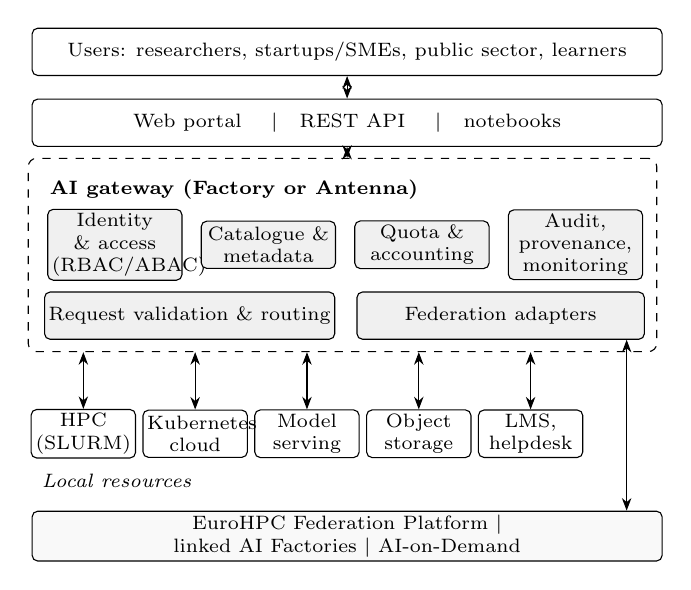
\begin{tikzpicture}[
  font=\scriptsize,
  box/.style={draw, rounded corners=2pt, align=center, minimum height=6mm, inner sep=1.5pt},
  core/.style={box, fill=gray!12},
  >={Stealth[length=1.6mm]}
]
\node[box, minimum width=8cm] (users) at (4,0) {Users: researchers, startups/SMEs, public sector, learners};
\node[box, minimum width=8cm] (portal) at (4,-0.9) {Web portal \quad\textbar\quad REST API \quad\textbar\quad notebooks};
\node[font=\scriptsize\bfseries, anchor=west] (gwt) at (0.1,-1.75) {AI gateway (Factory or Antenna)};
\node[core, text width=1.6cm] (iam)   at (1.05,-2.45) {Identity \& access\\(RBAC/ABAC)};
\node[core, text width=1.6cm] (cat)   at (3.0,-2.45) {Catalogue \&\\metadata};
\node[core, text width=1.6cm] (quota) at (4.95,-2.45) {Quota \&\\accounting};
\node[core, text width=1.6cm] (audit) at (6.9,-2.45) {Audit, provenance,\\monitoring};
\node[core, minimum width=3.65cm] (route) at (2.0,-3.35) {Request validation \& routing};
\node[core, minimum width=3.65cm] (fed)   at (5.95,-3.35) {Federation adapters};
\node[draw, dashed, rounded corners=3pt, fit=(gwt)(iam)(audit)(route)(fed), inner sep=1.5mm] (gw) {};
\foreach \n/\x/\t in {hpc/0.65/{HPC\\(SLURM)}, k8s/2.07/{Kubernetes\\cloud}, serve/3.49/{Model\\serving}, store/4.91/{Object\\storage}, lms/6.33/{LMS,\\helpdesk}}
  \node[box, minimum width=1.3cm, text width=1.22cm] (\n) at (\x,-4.85) {\t};
\node[font=\scriptsize\itshape, anchor=west] at (0,-5.45) {Local resources};
\node[box, minimum width=8cm, fill=gray!5, text width=7.8cm] (aif) at (4,-6.15) {EuroHPC Federation Platform \textbar\ linked AI Factories \textbar\ AI-on-Demand};
\draw[<->] (users) -- (portal);
\draw[<->] (portal) -- (portal |- gw.north);
\foreach \n in {hpc,k8s,serve,store,lms} \draw[<->] (gw.south -| \n) -- (\n);
\draw[<->] (7.55,-3.35 |- fed.south) -- (7.55,-3.35 |- aif.north);
\end{tikzpicture}
\caption{General model of an AI gateway between users, local resources and European AI Factory services.}
\label{fig:arch}
\end{figure}

The function groups in Table~\ref{tab:func} come from the SAIFA design (Section~\ref{sec:saifa}), where they were made from user stories and use cases. We wrote them in a general way, so they can be used by any Factory or Antenna. Three rules apply to all groups: the server checks permissions for every action, every result has a version and a record of where it came from, and every job is checked against the user's quota before it starts.

\begin{table}[t]
\centering
\caption{Main function groups of an AI gateway}
\label{tab:func}
\footnotesize
\renewcommand{\arraystretch}{1.1}
\begin{tabular}{@{}p{2.1cm}p{5.9cm}@{}}
\toprule
\textbf{Group} & \textbf{Main features} \\
\midrule
Identity \& access & Institutional (eduGAIN) and EuroHPC sign-in, account linking, RBAC/ABAC, scoped API tokens, revocation \\
Organisations \& projects & Workspaces, membership, roles, resource visibility (private, project, platform, public) \\
Catalogue & Search of models, datasets, workflows, services and courses; source attribution of federated entries \\
Data \& model management & Resumable upload, versioning, model and data cards, review and publication workflow \\
Compute jobs & Job templates, quota reservation, routing to HPC or Kubernetes, status, logs, result retrieval \\
Inference & Authenticated, rate-limited access to served models and LLMs \\
Experiments \& MLOps & Experiment tracking, run comparison, benchmark evaluation, lineage across job, dataset and model \\
Training & Courses, learning paths, preconfigured notebook labs with controlled resources \\
Operations & Monitoring, usage accounting, audit trail, notifications, contextual helpdesk tickets \\
Federation & Catalogue exchange, metadata mapping, identity brokering, cross-factory execution and accounting \\
\bottomrule
\end{tabular}
\end{table}

\begin{table*}[t]
\centering
\caption{Possible tools for each part and work needed for the gateway}
\label{tab:tools}
\footnotesize
\renewcommand{\arraystretch}{1.25}
\setlength{\tabcolsep}{4pt}
\newcommand{\grp}[1]{\multicolumn{3}{|l|}{\cellcolor{gray!12}\textbf{\textit{#1}}} \\ \hline}
\begin{tabular}{|>{\raggedright\arraybackslash}p{2.9cm}|>{\raggedright\arraybackslash}p{7.0cm}|>{\raggedright\arraybackslash}p{6.5cm}|}
\hline
\rowcolor{gray!30}
\textbf{Part} & \textbf{Main option (alternatives)} & \textbf{Work needed for the gateway} \\ \hline
\grp{User access}
Portal \& UX & Next.js/React (Nuxt/Vue) & Unified UI, backend-for-frontend, tool embedding \\ \hline
Identity \& policies & Keycloak (authentik, WSO2 IS); Open Policy Agent (Casbin, Cedar) & Role mapping, ABAC attributes, account linking, policy model \\ \hline
Notebooks & JupyterHub + KubeSpawner (SlurmSpawner, code-server) & Launch from portal, quotas, dataset mount, audit \\ \hline
\grp{Data and models}
Catalogue \& search & CKAN or Dataverse (DataHub, OpenMetadata); OpenSearch + pgvector & Unified catalogue, ACL filtering in index, federation \\ \hline
Model registry \& experiments & MLflow (ClearML, Aim) & Model cards, approval workflow, access rights \\ \hline
Storage & PostgreSQL, S3-compatible object store (MinIO/Ceph), Valkey & Metadata links, lifecycle, retention \\ \hline
Lineage & OpenLineage + Marquez & Links between jobs, datasets, models and results \\ \hline
\grp{Compute and inference}
LLM inference \& serving & vLLM (TGI, SGLang, Triton); KServe (Ray Serve, BentoML) & API proxy, quotas, routing, audit \\ \hline
Fine-tuning & Hugging Face TRL/PEFT (Axolotl, LLaMA-Factory) & Approved templates, HPC submission, result registration \\ \hline
HPC \& batch & SLURM, Open OnDemand; Kubernetes Jobs (Volcano, Kueue) & HPC bridge, unified job model, SLURM/K8s routing \\ \hline
Workflows \& containers & Argo Workflows (Airflow, Flyte); Harbor + Trivy, Apptainer on HPC & Workflow templates, image approval and HPC conversion \\ \hline
\grp{Operations and federation}
Observability \& audit & Prometheus, Grafana, Loki, OpenTelemetry; append-only log + WORM archive & Correlation with user/job, shared audit events \\ \hline
Learning \& support & Moodle (Open edX); Zammad or GLPI & Portal links, lab quotas, contextual tickets \\ \hline
Federation \& accounting & DCAT/DCAT-AP adapters (CKAN harvester); Waldur as cross-layer option & Partner adapters, per-factory accounting \\ \hline
\end{tabular}
\end{table*}

\section{Description of the Main Functions}

\subsection{Login, access and collaboration}
Users log in with their university or institute account (for example through eduGAIN) or with a EuroHPC account, and the gateway connects these logins to one user account. Access is decided by the user's role and by other attributes, such as organisation, project and type of data~\cite{nist_abac}. Seeing a resource in the catalogue and using it are two separate permissions. The search index also filters results, so users never see resources from other projects that they are not allowed to use.

\subsection{Datasets and models}
Datasets and models go through three steps: draft, review and publication. Review decisions are saved, and only checked versions that can no longer change can be used, published or shared. Large files are uploaded in parts with checksums. Published resources have FAIR metadata~\cite{wilkinson2016fair}, which also makes it easier to share them with partner catalogues.

\subsection{Jobs, inference and experiments}
Before a job starts, the gateway checks the input data and the user's access, and reserves quota. Then it sends the job to HPC through SLURM~\cite{yoo2003slurm} or to Kubernetes~\cite{burns2016borg}. Sensitive data can stay where it is, and the job is sent to the data. The scheduler still manages the queue. The gateway collects status, logs and results and shows them in the same way for all systems, and containers are converted to Apptainer/Singularity images~\cite{kurtzer2017singularity} for HPC. Requests to a model go through a proxy that checks the user and the limits and charges the quota before the request is sent on. Training and test runs are saved together with links to their data, jobs and benchmark versions. A person always decides which model to keep.

\subsection{Working with partners: Factory and Antenna}
Here the two roles differ the most. A Factory mostly \emph{publishes} its services and resources to European platforms. An Antenna also has to \emph{connect} its users with one or more linked Factories. It converts user identities and metadata, sends large test jobs to a partner site, returns the results to the user's project, and keeps track of usage for each Factory. Each partner is connected through its own catalogue adapter, for example using DCAT~\cite{w3c_dcat3}. Resources from partners keep their source and are never changed locally. The first connections are read-only or simulated, so the gateway keeps working when a partner is down. When AI Factories are added to the EFP~\cite{eurohpc_efp}, gateways should use its login and allocation services instead of building their own.

\section{Possible Tools and How to Choose Them}

The main rule is to use existing tools first and build new ones only when needed. Table~\ref{tab:tools} gives the main option for each part, alternatives in brackets, and the work that each gateway still has to do itself. Most options are well known open-source projects, for example JupyterHub~\cite{kluyver2016jupyter}, MLflow~\cite{zaharia2018mlflow}, vLLM~\cite{kwon2023vllm} and Open OnDemand~\cite{hudak2018ood}. New development is needed mainly for the portal, the common metadata model, the shared rules for access and quotas, audit and accounting, the HPC bridge and the partner adapters. Waldur is also worth considering, because one tool could cover the catalogue, resource allocation, accounting and HPC access. It should still be compared with a set of separate tools.

Tools are chosen in two steps. First, each tool must meet the basic requirements for its area. For example, it must let users log in through both SAML2 and OIDC and link these logins to one account, and it must be able to revoke a user's access immediately. The search must filter results by access rights. The model server must run behind the gateway, with quota charged before a request runs. Users must not need to work with SLURM directly, and a new partner must be added with a new adapter. Second, the tools that pass are compared by ease of use, work needed to connect them, effort to run them, speed and cost, maturity, and legal issues (GDPR, data location, licences). Open-source tools that can run on our own servers are preferred. Paid tools are noted, together with a plan to replace them if needed.

\section{Example: SAIFA}
\label{sec:saifa}

SAIFA is the Serbian Antenna, linked with Pharos and IT4LIA. The project runs from May 2026 to April 2029~\cite{cordis_saifa}. Its local resources are the PARADOX HPC cluster at the Institute of Physics Belgrade and the AI infrastructure of the Institute for AI Research and Development of Serbia. It focuses on four domains: language and culture, energy and manufacturing, health, and environment. The function groups in Table~\ref{tab:func} were made from 23 user stories, such as flood prediction with AutoML, synthetic genome sequencing data, hate-speech detection in Serbian and simulation of social networks with LLM agents. These stories were then turned into 20 system use cases~\cite{saifa_d31}.

The SAIFA design proposes a basic proof-of-concept setup to test the selected tools together: a web portal, login through home institutions, an access-control module, PostgreSQL with S3 storage, JupyterHub, a model-serving service, a separate bridge to SLURM, and Prometheus/Grafana monitoring. For each part, the proof of concept must show where the data is stored, how the user identity is passed on, how resources are charged, how actions are logged, how access is checked and what happens when another service fails~\cite{saifa_d31}. The beta version of the gateway is planned for April 2027 and must offer at least one full path for a user: log in, find a resource, run a job and follow its progress. Final tests and benchmarks are planned on the Greek and Italian Factories.

\section{Conclusion}

The AI Factory network already offers computing, services and shared European platforms. Users still need one place where they can use all of this in their daily work. The model in this paper describes such a gateway. It sits between users and existing systems, has clearly defined tasks, can be used by both Factories and Antennas, and can be built mostly from existing open-source tools. Some questions are still open: how gateways will use the EFP for login and allocation, how to track usage across several Factories, which common metadata to use for sharing models and datasets, and which data rules apply when jobs run in another country. Next, we will report on the SAIFA beta version and on tests with Pharos and IT4LIA.

\bibliographystyle{IEEEtran}
\bibliography{references_v2}

\end{document}
